\chapter{Revisão sistemática}
\label{capitulo3}
Uma revisão sistemática da literatura é um meio de identificar, avaliar e interpretar
toda a pesquisa disponível relevante para uma questão de pesquisa em particular, ou área temática, ou
fenômeno de interesse \citeonline{kitchenham2004procedures}. 


Desta forma, a metodologia deste trabalho é
baseada no método exposto por \cite{kitchenham2004procedures},
que é apresentado em 3 etapas principais:

\begin{enumerate}
    \item \textbf{Definir questões de pesquisa;}
    \item \textbf{Realizar a busca de estudos primários
e seleção dos estudos relevantes}: São todos os estudos encontrados como resultado à aplicação
da string de busca nas bases de dados \cite{kitchenham2004procedures}
    \item \textbf{Extrair dados e analisar os resultados}: São os estudos resultantes da aplicação dos critérios de
inclusão e exclusão que são relevantes para responder as
questões de pesquisa \cite{kitchenham2004procedures}
\end{enumerate}

As etapas dessa metodologia são
ilustrada na figura \ref{fig:fig0}. 

\begin{figure}[H]
  \caption{Fluxograma das etapas da revisão}

  \centering
  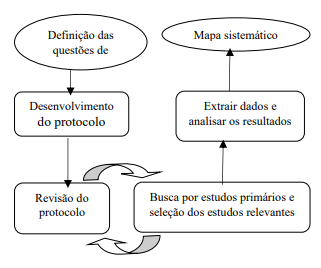
\includegraphics[scale=1.0]{Imagens/mapeamento.png} 
  
  \legend{Fonte: Adaptado de \cite{kitchenham2004procedures}
  }
  \label{fig:fig0}
\end{figure}

\subsection{Planejamento da revisão}

Nesta primeira fase de planejamento, será informado o propósito e os objetivos do
trabalho; as fontes, estratégias e questões de pesquisa; os critérios e procedimentos de seleção
dos resultados; e a forma de extração dos dados destes resultados.

\subsubsection{Questões de pesquisa}
Segundo \cite{kitchenham2004procedures}, formular as questões de pesquisa é a atividade de maior importância ao realizar uma revisão sistemática. Além disso,
as questões de pesquisa visam descobrir tendências de pesquisa (p.ex., tendência de publicação ao longo do tempo, tópicos cobertos na literatura etc.) \cite{Kraemer:2007:HFS:1289816.1289837,kitchenham2004procedures,petersen2008systematic}. Dessa forma, as seguintes questões de pesquisa foram estabelidas:


\begin{enumerate}
     \item[Q1.] Quais frameworks são usadas atualmente desenvolver chatbots ?
    \item[Q2.] Quantas Frameworks são open source ?
    \item[Q3.] Qual o custo de utilização dessas frameworks ?
    \item[Q4.] Quais frameworks realizam processamento de linguagem natural ?
    \item[Q5.] Quais são as características destas frameworks ?
\end{enumerate}

\subsubsection{Estratégias de busca }
Esta seção descreve as fontes de pesquisa e como foram realizadas as buscas, bem como as palavras-chave
que geraram a string de busca e as línguas aceitas para os resultados selecionados.

Foram selecionadas cinco bases bibliográficas, nas quais foi realizada a busca por estes
trabalhos, esta atividade foi realizada no mês de janeiro de 2019 e os resultados retornados
correspondem ao que tinha disponível até esta data.

Para este mapeamento foram utilizadas as seguintes
bases de dados: Scopus, IEEE, science direct, webof science, conpendex e ACM.

\subsubsection{Critérios de Seleção}
De acordo com as questões de pesquisa e com o objetivo da revisão foram definidos
critérios de inclusão e exclusão relevantes para o tema da pesquisa, com o objetivo de nortear a
seleção dos artigos na fase de condução da revisão. Foram elaborados 4 critérios de inclusão (I)
e 4 critérios de exclusão (E) como apresentados abaixo.

Os critérios de inclusão considerados na seleção dos artigos:

\begin{itemize}
    \item I1. O artigo possui informações pertinentes ao escopo do trabalho a exemplo pesquisas de interesse e dados relacionados a frameworks ou plataformas de desenvolvimento de chatbots.
        \item I1. O artigo apresenta alguma ferramenta ou método para desenvolvimento de chatbots.
    
\end{itemize}

Os critérios de exclusão considerados na seleção dos artigos:

\begin{itemize}

    \item E1. No artigo a temática de frameworks para desenvolvimento de chatbots não é abordada.
    \item E2. O artigo apresenta alguma aplicação ou desenvolvimento de chatbots específicos.
    
\end{itemize}

\subsubsection{String de Busca}
Como etapa final do planejamento da revisão foi definida uma string de busca. Para
este fim foram consideradas as palavras chaves do assunto de interesse e seus sinônimos como
apresentados na tabela \ref{tab:termosBusca}.



\begin{table}[H]
    
    \begin{center}
    \begin{tabular}{||c c||} 
    \hline
    Termos & Sinônimos \\ [0.5ex] 
    \hline
    Bot & Chatbot, Chat-bot, Chatterbot   \\ 
    \hline
    Framework & Platform  \\
    \hline
    Development & Building \\
    \hline
    \end{tabular}
    \caption{Termos e sinônimos.}
    \label{tab:termosBusca}
    
    \end{center}
   
\end{table}


Com os termos da pesquisa definidos e utilizando os operadores booleanos <AND> (E) e
<OR> (OU) foi elaborada uma string genérica de busca (Tabela \ref{tab:stringGenerica}), a qual foi utilizada nas bases
bibliográficas durante a seleção dos artigos.

\begin{table}[H]
    
    \begin{center}
    \begin{tabular}{| c |} 
    \hline
    (bot OR chatbot OR chat-bot OR chatterbots) AND (building platform OR development framework) \\ 
    \hline
    \end{tabular}
    \caption{String genérica de busca.}
    \label{tab:stringGenerica}
    
    \end{center}
   
\end{table}


\subsection{Seleção dos estudos primários}

Utilizando a string genérica e alguns filtros nas diferentes bases, foram coletados os
artigos de interesse para o trabalho. Determinou-se um período limite em algumas bases para
refinar os resultados de forma que fossem retornados os artigos mais recentes, para isso foi
definido um filtro de data a partir de anos maiores que 2015 para a Science Direct, de 2000 a
2018 para a IEEE e Scopus, e por fim 2014 a 2019 para a Web of Science.
As strings geradas em cada base de acordo com as entradas utilizadas são as especificadas na
tabela \ref{tab:stringBase}.


\begin{table}[H]
    
    \begin{center}
    \begin{tabular}{| p{5cm}| p{10cm}|}
    \hline
     Base & String\\
    \hline
     Science direct & (chatbot OR chatterbots) AND (development framework)
Filters Applied: 2015-2019 \\ 
    \hline
     IEEE & (bot OR chatbot OR chat-bot OR chatterbots) AND (building platform OR development framework)
Filters Applied: 2000-2018\\ 
    \hline
     Scopus & (bot OR chatbot OR chat-bot OR chatterbots) AND (building platform OR development framework)Filters Applied: nenhum mas trouxe resultados entre 2002-2018\\ 
    \hline
     Web of science & (bot OR chatbot OR chat-bot OR chatterbots) AND (building platform OR development framework) Filters Applied: Últimos 5 anos. Índices: SCI-EXPANDED, SSCI, A\&HCI, CPCI-S, CPCI-SSH, ESCI.\\
     \hline
    \end{tabular}
    \caption{ String de busca de cada base.}
    \label{tab:stringBase}
    
    \end{center}
   
\end{table}

Dessa forma a distribuição de artigos por base ficou como apresentado na figura \ref{fig:bases}, sendo
a IEEE com 58 artigos, a base com o maior número de resultados, seguido da
Science direct com 57, Web of science com 48 artigos, por fim com o menor
número de resultados o Scopus com 13 artigos.


\begin{figure}[H]
  \caption{Quantidade de Artigos coletados por base}

  \centering
  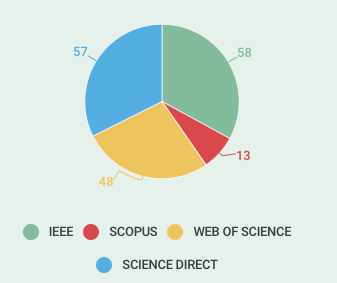
\includegraphics[scale=0.8]{Imagens/grafico_bases.png} 

  \label{fig:bases}
  Fonte: O autor
\end{figure}

O processo de seleção se caracterizou em etapas. Inicialmente foram baixados os arquivos
bibtex de todos os artigos retornados pelas bases através da \textit{string} de busca inserida, para então começar o
processo de seleção. 

No processo de seleção foram lidos os títulos, resumos e palavras-chave para então serem
escolhidos os artigos que foram relevantes de acordo com os critérios. Uma vez que esta pré-seleção foi realizada, foram separados 12 artigos para serem analisados mais
profundamente, explorando mais do seu conteúdo.

Após a leitura dos 12 artigos selecionados para extração de características foi constatado que nenhum atendia as características desejadas, já que não tratavam de \textit{frameworks} para desenvolvimento, mas soluções específicas de \textit{chatbots} ou algoritmos. Esse resultado sugere que esse tipo \textit{framework} não é um tema abordado e publicado nas bases pesquisadas.


\section{ Revisão de Produtos do Mercado}
Não apenas os artigos foram analisados, como também as ferramentas existentes no
mercado para desenvolvimento de chatbots. Um processo de seleção semelhante ao dos
artigos aconteceu na Revisão de Produtos no Mercado, na qual a partir de diferentes strings de
busca inseridas na ferramenta de pesquisa da Google uma lista de frameworks foi
selecionada. Das 33 frameworks que foram retornados nas buscas, 14 open source foram escolhidos para uma
análise mais aprofundada e por fim 4 foram tomados como referência para o produto de software
desenvolvido neste trabalho.


Uma pesquisa na plataforma stack overflow\footnote{O Stackoverflow é um website de perguntas e respostas, criado em 2008, mundialmente usado por desenvolvedores, engenheiros de software e pesquisadores para compartilhar conhecimento e sanar dúvidas relacionadas a tecnologia e outras áreas. Website: https://stackoverflow.com} foi realizada estabelecer um indicativo de que tais frameworks ou plataformas estão em uso na comunidade de desenvolvedores e no mercado. A figura \ref{fig:frameworks} representa a quantidade de perguntas relacionadas a cada framework.


\begin{figure}[H]
  \caption{Quantidade de perguntas em cada framework no stackoverflow}

  \centering
  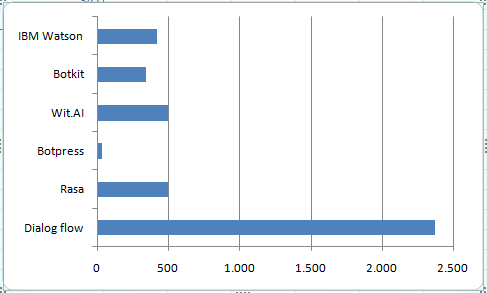
\includegraphics[scale=1]{Imagens/frameworks-stack.png} 

  \label{fig:frameworks}
  Fonte: O autor
\end{figure}

Devido a alta popularidade, o IBM Watson Assistant e Dialog Flow foram selecionados para uma comparação apesar de não serem open source. Vale ressaltar que o Botpress e IBM Watson possuem suas próprias áreas de perguntas onde a comunidade de desenvolvedores interage. 


\begin{itemize}
    \item Botpres \footnote{Fórum em :https://help.botpress.io/top}: 383 perguntas
    \item IBM Watson Assistant \footnote{Fórum em: https://developer.ibm.com/answers/smartspace/watson/index.html}: 4063 perguntas 
\end{itemize}



O Quadro apresenta as frameworks analisados e os URls para acesso a estas. Além disso, responde a primeira questão de pesquisa.

Quais frameworks open source são usadas atualmente desenvolver chatbots ?


\begin{table}[H]
    
    \begin{center}
    \begin{tabular}{| p{3cm}| p{3cm}|  p{3cm}|}
    \hline
     Framework & URL & Licensa\\
    \hline
    Rasa & https://rasa.com/ & Apache 2.0 \\
    \hline
    Wit.ai & https://wit.ai/ & MIT License \\
    \hline
    Botpress & https://botpress.io/ &  AGPLv3 e Licensa proprietária Botpress \\
    \hline
    Botkit & https://botkit.ai/ & MIT license \\
    \hline
    
    \end{tabular}
    \caption{ Frameworks e respectivas urls e licensas}
    
    \end{center}
   
\end{table}

As seções seguintes descrevem o que foi encontrado na exploração destas frameworks, apresentando como cada uma delas funciona.


\subsection{Rasa}

A framework Rasa ou Rasa Stack possui um conjunto de ferramentas de aprendizado de máquina para que desenvolvedores possam criar chatbots contextuais, diferente de daqueles baseados em regras pré-definidas. Essa framework é composta de dois módulos que são independentes e podem ser usados separadamente. O módulo principal (Rasa Core) e módulo de processamento de linguagem natural (chamado de Rasa natural language understanding ou Rasa NLU) são detalhados a seguir:

\begin{enumerate}
    \item Rasa Core (Núcleo): È uma ferramenta que usa aprendizado de máquina para inferir possíveis ações a serem executadas pelo chatbot. O aprendizado de máquina é feito com o constante feedback do usuário, e a partir disso, são calculadas as probabilidades de execução de cada ação. Essa abordagem é conhecida como aprendizado iterativo.
    \item Rasa NLU: È uma ferramenta para processamento de linguaguem natural open source capaz de classificar intenções dos usuários e extrair entidadades em chatbots. Sendo assim, é possível extrair dados estruturados de uma conversa em linguagem natural. Vale ressaltar que esse módulo pode ser executado em qualquer ambiente sem depender de chamadas á api's externas como as do Google, IBM Watson ou Microsoft.
    
\end{enumerate}

A integração com canais de comunicação nessa framework é possível de forma programática nos seguintes canais:

\begin{itemize}
    \item Web
    \item Facebook Messenger
    \item Slack
    \item Twilio
    \item Google Hangouts\footnote{https://hangouts.google.com}
    \item Microsoft Teams\footnote{https://products.office.com/pt-br/microsoft-teams}
    \item Webex Teams\footnote{https://www.webex.com}
    \item Conectores customizados
\end{itemize}



\subsection{Wit.ai}

Wit.ai é uma plataforma que implementa uma API (do inglês application program interface) gratuita para instancias públicas e privadas sem limitações para requisições. Fornece reconhecimento de voz e texto por meio do apredizado de máquina. Além disso, possui elementos como a classificação de intenções e extração de entidades. Também disponibiliza entidades pré-definidas como temperaturas, números, email e outras entidades comumente utilizadas em chatbots.

Essa plataforma foi adquirida pelo facebook em 2015 e, portanto, pode ser integrado com mais facilidade com o facebook messenger. O algoritmo de apredizado dessa plataforma é baseado em histórias (casos de uso dependentes de domínio). Além disso, Essa plataforma possui inteface de programação gráfica, possibilitando assim que usuários sem conhecimento de programação possam desenvolver chatbots. 

A desvantagem do Wit.ai é o fato ser uma solução hospedada pelo facebook onde os recursos são centralizados e somente disponíveis via requisições http. Além do mais, só permite integração com o Facebook Messenger.


\subsection{Botpres}
Botpres é uma framework que possibilita a integração com as principais plataformas de mensagens como Telegram, facebook messenger, slack e etc. A arquitetura dessa framework é modular, ou seja, permite a integração com módulos internos, externos, ou módulos criados e personalizados pelo desenvolvedor. A proposta da framework é fornecer um ambiente para a criação de novos módulos que podem ser integrados como plugins wordpress \footnote{WordPress é um sistema livre e aberto de gestão de conteúdo para internet, baseado em PHP com banco de dados MySQL, executado em um servidor interpretador, voltado principalmente para a criação de páginas eletrônicas e blogs online.} (De fato, o wordpress para chatbots).

Outras funcionalidades são gerenciamento do fluxo conversacional via interface, suporte ao processamento de várias linguagens, ferramenta para análise estatísticas e a possibilidade de intervenção humana quando o chatbot não consegue resolver ou entender algum problema. Além disso, possui uma estrutura que facilita a integração nos seguintes canais:

\begin{itemize}
    \item Web
    \item Facebook Messenger
    \item Slack
    \item Microsoft Teams\footnote{https://products.office.com/pt-br/microsoft-teams}
\end{itemize}

\subsubsection{Tabela de preços}

Apesar de ser \textit{open source}, a proposta do Botpress atualmente é que somente grandes empresas serão cobradas pelo uso da \textit{framework}. No futuro serviços e ferramentas \textit{premium} também serão ofertadas e cobradas. A figura \ref{fig:bot-planos} apresenta os planos.

\begin{figure}[H]
  \caption{Planos da framework botpress}

  \centering
  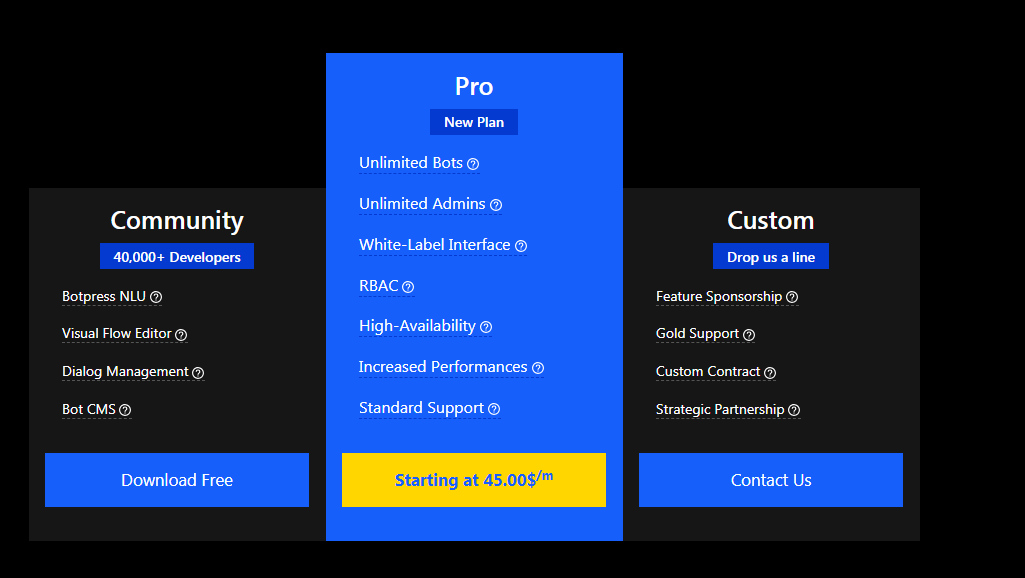
\includegraphics[scale=0.5]{Imagens/botpress-precos.png} 
 
  \label{fig:bot-planos}
  Fonte: https://botpress.io/pricing
\end{figure}



\subsection{Botkit}

É uma framework open source que foi adquidira pela Microsoft em novembro de 2018. Essa framework disponibiliza nativamente funcões de desenvolvimento de chatbots simples e baseados em regras. Entrentanto, a principal vantagem é a flexibilidade de utilizar essa framework em conjunto com outras que possuem métodos de processamento de linguagem natural para atribuir maior inteligencia ao conversador. Além disso, possui uma estrutura que facilita a integração nos seguintes canais:

\begin{itemize}
    \item Web
    \item Facebook Messenger
    \item Slack
    \item Twilio
    \item Google Hangouts\footnote{https://hangouts.google.com}
    \item Microsoft Teams\footnote{https://products.office.com/pt-br/microsoft-teams}
    \item Webex Teams\footnote{https://www.webex.com}
\end{itemize}


Devido a aquisição da framework pela Microsoft o site oficial recomenda a utilização do botkit com ferramentas de processamento de linguagem natural  da empresa, Luis.ai. Além disso,  a integração de um chatbot construido com o botkit em outros canais de comunicação como Telegram e whatsapp é recomendada utiliazando o Microsoft Bot Framework\footnote{https://dev.botframework.com/} onde também é possível realizar análise estatísticas das conversas realizadas no chatbot. O uso dos recursos essa framework Microsoft é pago, porém é possivel utilizar somente o botkit de forma independente.

\subsection{IBM Watson}

O IBM Watson é uma plataforma que oferece serviços de computação cognitiva. A IBM lançou a plataforma em 2011 e o nome é em homenagem ao  CEO Thomas J. Watson.

A computação cognitiva é uma mistura de diversas técnicas como processamento de linguagem natural, aprendizado de máquina, inteligencia artificial e etc. Também possui serviços como reconhecimento e análise de vídeos e imagem; interação por voz; leitura de grandes volumes de textos.

O IBM Watson é uma plataforma que oferece outros serviços na nuvem, entretanto, para o desenvolvimento de chatbots é utilizado o Watson Assistent.

As características do Watson Assistent são:


\begin{itemize}
    \item Conteúdo pré-construído: Adicione atendimento ao cliente e outros pacotes específicos de cada área (finança, saúde, etc) prontos para iniciar seu assistente.
    \item Desambiguação: Quando uma requisição do usuário não está clara, o Watson irá automaticamente propor múltiplos opções em vez de responder incorretamente.
    \item Resolução de conflitos de Intenção:
Uso de inteligência artificial para identificar erros introduzidos por humanos nos dados de treinamento.
    \item Recomendação de Intenção: Uso dos dados de conversas existentes para treinar o assistente mais rápido.
    \item Habilidade de Busca: Realiza busca em dados desestruturados para ampliar o conhecimento do assistente
    
    \item Linguagem natural: Processa linguagem natural e realiza conversão tanto de voz para texto quanto de texto para voz.

\end{itemize}


A possibilidade de integração em diversos canais é facilitada por essas plataforma pois essa funcionalidade é entregada ao desenvolvedor a partir do preenchimento de alguns formulários simples com informações sobre o canal. Alias um grande diferencial é que além dos canais convencionais é feita integração com dispositivos IOT\footnote{Internet das coisas, em inglês Internet of Things (IOT)}.


\subsubsection{Tabela de Preços}

Os custos relacionados ao uso da plataforma dependem do plano e recursos demandados. Existe um plano gratuido que dura um mês para testar a plataforma e após esse período precisa ser migrado para algum dos outros planos pagos. As figuras \ref{fig:basico} e \ref{fig:avancado} apresentam mais detalhes sobre os planos. 



\begin{figure}[H]
  \caption{Planos básicos da plataforma IBM Watson Assistant}

  \centering
  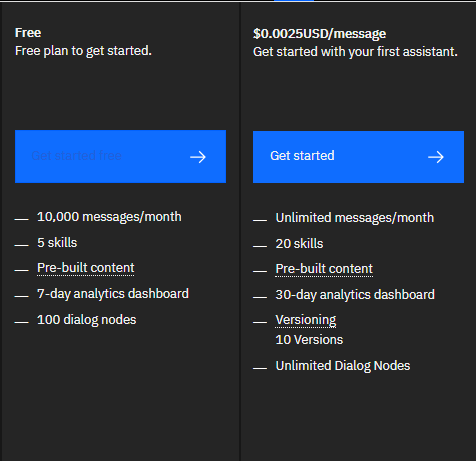
\includegraphics[scale=0.5]{Imagens/ibm-basic.png} 
 
  \label{fig:basico}
  
  Fonte: https://www.ibm.com/cloud/watson-assistant/pricing/
\end{figure}



\begin{figure}[H]
  \caption{Planos avançados da plataforma IBM Watson Assistant}

  \centering
  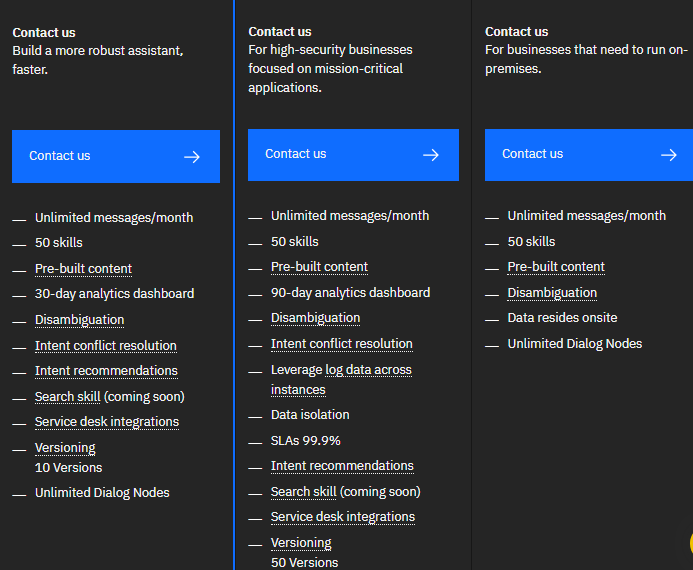
\includegraphics[scale=0.5]{Imagens/ibm-other.png} 
 
  \label{fig:avancado}
    Fonte: https://www.ibm.com/cloud/watson-assistant/pricing/
\end{figure}



Para a maioria das aplicações o plano lite parece ser adequado, entretanto, quando existe a necessidade de utilizar outros recursos é preciso entrar em contato com a IBM para que se possa obter um orçamento dos custos. 

A tabela \ref{tabela:simulacaoIBM} foi elabora para fornecer uma visão geral dos custo associados ao uso da plataforma da IBM.


\begin{table}[H]
    
    \begin{center}
    \begin{tabular}{| p{3cm}| p{3cm} | p{3cm}|}
     \hline
      N° Mensagens & USD & Real\\
    \hline
     2.000 & 5,00 &  18,68 \\
    
    \hline
     5.000 & 12,5 & 45,62  \\
    
    \hline
     10.000 & 25,00 & 93,25 \\
    
    \hline
     30.000 & 75,00 & 279,75\\
    \hline
   
   
    \end{tabular}
    \caption{Simulação de preços baseada no plano Lite do IBM Watson Assistant}
    \label{tabela:simulacaoIBM}
    \end{center}
   
\end{table}


\subsection{Dialog Flow}

Dialog Flow é uma plataforma do google, antes chamada de API.AI, que fornece ferramentas para processamento de conversas em linguagem natural. 

A principais características dessas plataforma são :

\begin{itemize}
    \item Processamento de Linguagem Natural: Processamento de dados em linguagem natural e classificação de intenção e entidades
    \item Aprendizado de máquina: Uso de dados para treinamento e melhora da interação aplicada ao domínio do problema
    \item Contexto: Controle do estado atual, ou dados , das conversas com os usuários. Esses dados podem ser usados como input ou output para eventos ou qualquer eventual processamento.
    \item Pode ser integrado com qualquer plataforma de mensageiros como Facebok, slack etc. Além de ser integrável com dispositivos móveis e weareables.
    \item Análise estatística dos dados 
\end{itemize}

Além disso, uma vantagem distinta do Dialogflow é o seu programa de análise, chamado de chatbase. O Google já é um elemento importante da análise da web e de usuários, graças à sua plataforma do Google Analytics \footnote{https://analytics.google.com/analytics/} estabelecida há muito tempo. 

 As integrações em um clique no Dialogflow, é possível gerenciar a integração do agente com o Google Assistente por meio do Actions on Google e muitas outras plataformas de mensagens famosas, como o Slack, o Facebook Messenger e o Twitter. Além disso, o Dialogflow facilita a exportação ou importação de agentes de/para outras plataformas de processamento de linguagem natural, como o Amazon Alexa e o Microsoft Cortana.


\subsubsection{Tabela de preços}

O Dialog Flow possui um plano gratuito porém com funções limitadas e outro pago para empresas. Os preços e características de cada plano são apresentados na figura \ref{fig:dialog-precos}.



\begin{figure}[H]
  \caption{Planos da plataforma Dialog Flow}

  \centering
  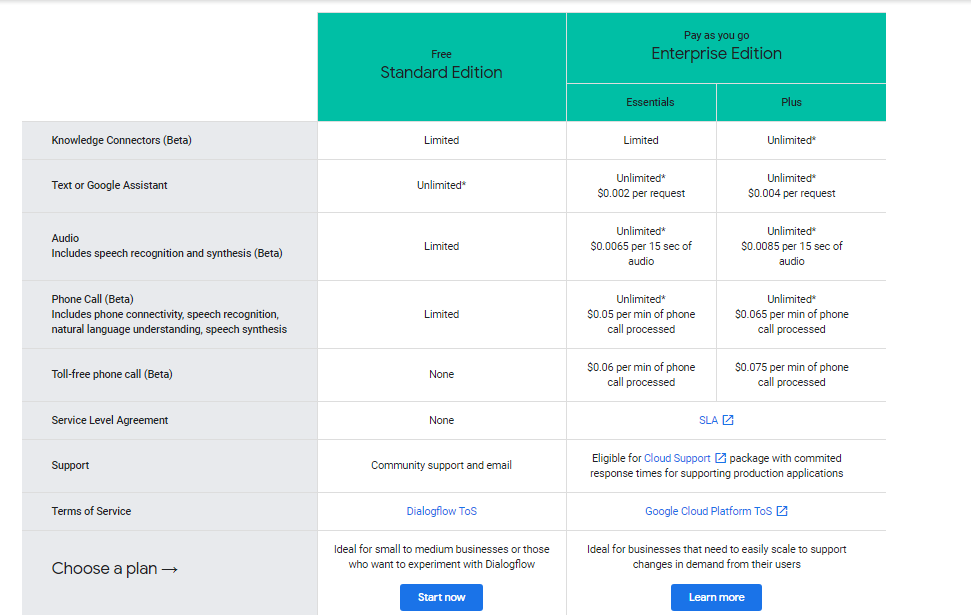
\includegraphics[scale=0.5]{Imagens/dialog-precos.png} 
 
  \label{fig:dialog-precos}
  
  Fonte: https://cloud.google.com/dialogflow/pricing
\end{figure}




\subsection{Extração de características}

A partir da exploração dos 4 aplicativos 7 características foram extraídas. As principais características encontradas nas frameworks estão discriminadas no Quadro \ref{tabela:caracteristicas}, assim como suas respectivas identificações.

\begin{table}[H]
    
    \begin{center}
    \begin{tabular}{| p{5cm}| p{5cm}|}
    \hline
     Identificação & Características\\
    \hline
    C1 & Open source\\
    \hline
    C2 & Integração com mensageiros externos \\
    \hline
    C3 &  Processa linguagem natural\\
    \hline
    C4 & Usa aprendizado de maquina para inferir contexto \\
    \hline
    C5 & Processa áudio \\
    \hline
    C6 & Fornece interface  gráfica \\
    \hline
    C7 & Realiza análise estatística \\
    \hline
   
    \end{tabular}
    \caption{ Principais características identificadas nas frameworks}
    \label{tabela:caracteristicas}
    \end{center}
   
\end{table}

A partir do levantamento destas características foi construído um quadro associando estas a cada uma das frameworks. O Quadro \ref{tabela:comparativo} exibe quais característica são apresentadas por cada framework, respondendo assim, a segunda e terceira questão de pesquisa.

Quais frameworks realizam processamento de linguagem natural ?

Quais são as características destas frameworks?


\begin{table}[H]
    
    \begin{center}
    \begin{tabular}{| p{2cm}| p{1cm}| p{1cm} | p{1cm}| p{1cm}| p{1cm}| p{1cm}| p{1cm}|}
     \hline
       & C1 & C2 & C3 & C4 & C5 & C6 & C7\\
    \hline
     Dialog Flow &  &   & X & X & X  &  &  \\
     \hline
     Watson Assistant &  &   & X & X &   &  &  \\
    
    \hline
     Rasa & X &   & X & X &   &  &  \\
    
    \hline
     Wit.ai & X &   & X & X & X &  &  \\
    
    \hline
     Botpress & X & X & X &  &   & X & X\\
    
    \hline
     Botkit & X & X &   &   & X & X & X\\
    
   \hline
   
    \end{tabular}
    \caption{ Principais características identificadas nas frameworks}
    \label{tabela:comparativo}
    \end{center}
   
\end{table}


\subsection{Escolha das Frameworks}


Decidir qual framework será mais adequada para um projeto de software não é tarefa trivial. Em seu famoso artigo \textit{“No Silver Bullet — Essence and Accident in Software Engineering"} (Não há bala de prata — Essência e Acidente na Engenharia de Software em português), Frederick P. Brooks afirmou, em 1986, que não existe nenhuma metodologia de desenvolvimento ou técnicas de gestão que consiga aumentar significativamente a produtividade e confiabilidade da engenharia de software. Assim, de forma analoga, não existe a framework perfeita e, portanto, a escolha da mesma deve levar em conta os requisitos e restrições do projeto em questão.

Sendo assim, os requisitos gerais e suficientemente amplos de forma que sirvam de referência para este trabalho e projetos futuros. Esse requisitos gerais também podem ser entendidos como recursos ou habilidades que um chatbot necessita e que a framework escolhida deve prover. Também é possivel que se utilize mais de uma framework para atender os requisitos do projeto.


\begin{itemize}
    \item \textbf{NLP: } O chatbot deve ter um módulo de processamento de linguagem natural
    \item\textbf{ IA:}  O chatbot deve possuir algoritmos de aprendizado de máquina para que possa entender contextos de conversação e ampliar sua base de conhecimento.
    \item \textbf{Canais: } O chatbot deve estar presente em mais de um canal de comunicação
    \item\textbf{ Hospedagem:}  O chatbot não deve depender de um serviço de hospedagem específico podendo ser hospedado em qualquer infraestrutura disponível e de acordo com as restrições orçamentárias do projeto. 
    
\end{itemize}

Vale ressaltar que um outro critério importante a se considerar na escolha da framework é o tamanho da comunidade que a mantém atualizada e realiza correções frequentes. Nesse ponto, todas as frameworks selecionadas na fase de levantamento possuem comunidade ativa.  

A partir dos critérios selecionados as frameworks Botkit e Rasa foram selecionadas. O diagrama da figura \ref{fig:frame-decisao} ilustra o processo de tomada de decisão.

\begin{figure}[H]
  \caption{Diagrama ilustrativo do processo de escolha das frameworks de desenvolvimento.}

  \centering
  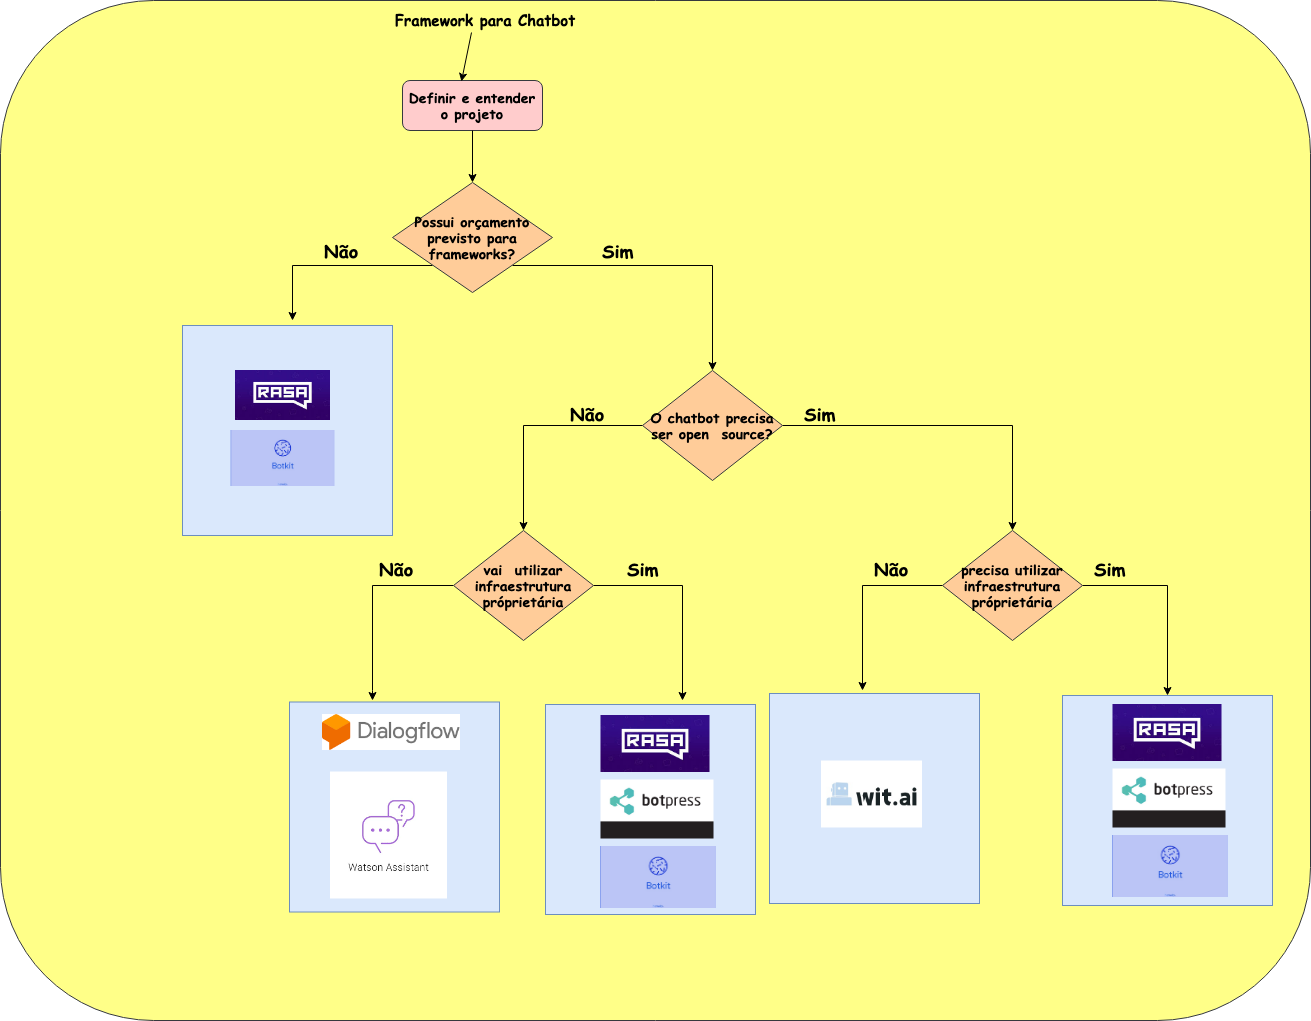
\includegraphics[scale=0.37]{Imagens/decisao_frame.png} 
  \label{fig:frame-decisao}
  Fonte: O autor.
\end{figure}



As frameworks Botkit e Rasa com o objetivo de abranger todas as 7 características definidas. Essas frameworks permitem que as soluções desenvolvidas sejam escaláveis, uma vez que fornece total domínio dos dados e do código interno, são independentes de infraestrutura e permitem integração em múltiplos canais. 

As frameworks Dialog Flow, IBM Watson Assistant e Wit.ai são altamente dependentes de serviços hospedados em servidores proprietários. Portanto, possuem limitações em termos custos, domínio dos dados de aplicações e escalabilidade. 




